\section{Continuous Integration overview}

\begin{frame}{Continuous Integration of Scientific Software}
    \framesubtitle{Benefits of Continuous Integration} 

    \epigraph{"Après moi, le déluge" - "After me, the flood"}{\href{https://en.wikipedia.org/wiki/Apr\%C3\%A8s_moi,_le_d\%C3\%A9luge}{Louis XV of France}}

    Even if you are not "Betty" yourself, and you or your supervisor don't really care what happens as long as papers are published, \textbf{Continuous Integration pays off quickly and speeds up research!}
    \begin{itemize}
        \item \textbf{CI is for your workflow, what a script with a for-loop is for starting a parameter study: it takes a day or two to set up, and pays off after you run it a couple of times.}
        \item \textbf{CI makes it possible to quickly test and compare different methods.}
        \item \textbf{CI simplifies the re-use of previous research (data, methods, and algorithms).}
    \end{itemize}

\end{frame}

\begin{frame}{(Continuous Integration with result visualization)} 
	\framesubtitle{Schematic diagram}

	\centering
	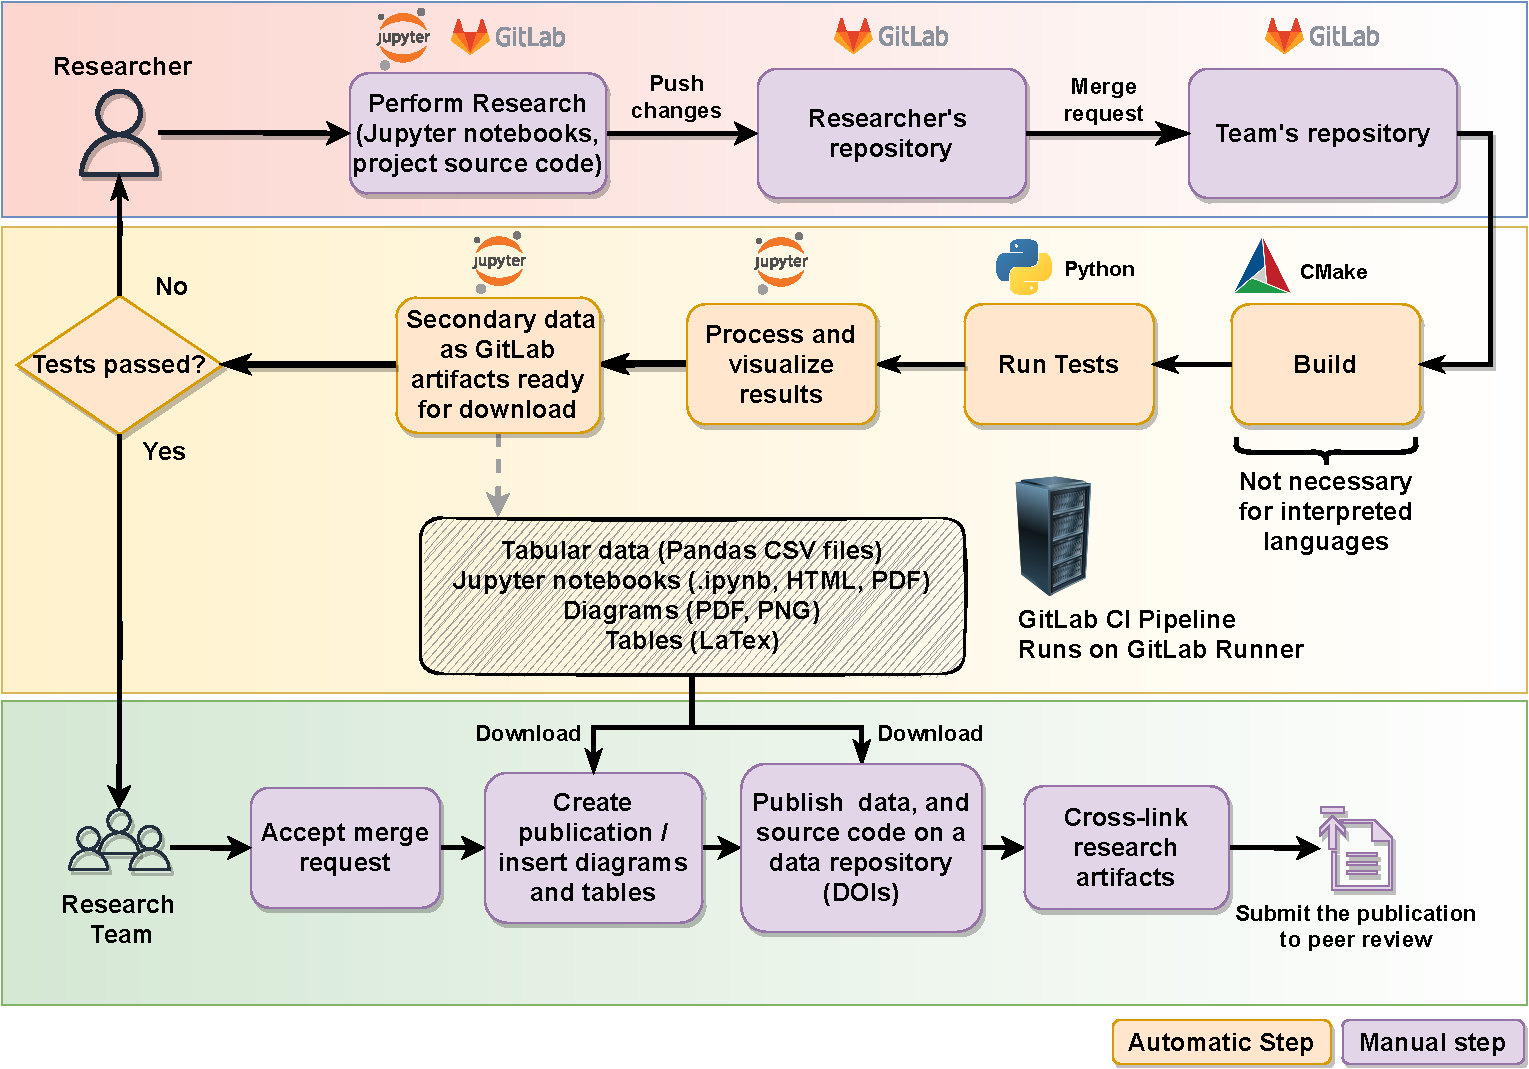
\includegraphics[width=0.8\textwidth]{figures/ZINF-CI-diagram.pdf}

\end{frame}

\begin{frame}{(Continuous Integration with result visualization)} 
    \framesubtitle{Testing machines and test categorization}

    \vfill
    \begin{enumerate}
        \item \textbf{Short few CPU-core tests}: work-PC \faGraduationCap.    
        \item \textbf{Short many-core tests}: obtain a workstation with a 64-Core CPU\footnote{Thanks to \href{https://www.sfb1194.tu-darmstadt.de/index.en.jsp}{CRC 1194 at TU Darmstadt.}}\faGraduationCap.
        \item \textbf{HPC tests}: combine 1. or 2. with an HPC cluster. 
    \end{enumerate}

    An HPC cluster is relevant for production tests and performance measurements.
    \begin{itemize}
        \item This workflow uses coarse ("smoke") tests \faGraduationCap
            \begin{itemize}
                \item Unit tests run for 1. and 2.
                \item Convergence ensured for 1. and 2.
                \item Is efficient in parallel for 1. and 2. 
            \end{itemize}
        \item \textbf{Challenge}: Is it possible to combine 1., 2. and 3. and publish instead of perish \faGraduationCap?
    \end{itemize}

\end{frame}


\begin{frame}{(Continuous Integration with result visualization)} 
    \framesubtitle{A GitLab runner with a Docker executor and a local Docker image}

    \vfill 
    Build a Docker image for your software, and track the Dockerfile with the project.\\
    \medskip
    \href{https://gitlab.com/tmaric/fvc-reconstruct/-/tree/main/docker}{Example OpenFOAM Dockerfile} on \texttt{ubuntu:focal} with "system" open-mpi and scotch.

    \medskip
    On the testing machine
    \begin{itemize}
        \item Install Docker and GitLab runner and register the GitLab runner with a Docker executor.
        \item Configure the GitLab runner in \texttt{/etc/gitlab-runner/config.toml} to
            \begin{itemize}
                \item use a local Docker image, e.g., \texttt{image = "openfoam-v2012\_ubuntu-focal:latest"}, and
                \item never pull images \texttt{pull\_policy = never}.
            \end{itemize}
    \end{itemize}


\end{frame}

\begin{frame}{(Continuous Integration with result visualization)} 
    \framesubtitle{Building}

    \vfill
    \begin{itemize}
        \item Files created within a job are gone when the job ends. 
        \item GitLab uses \textbf{job artifacts} to pass on data from one job to the next. 
        \item \textbf{Job artifacts only work with files stored in project's sub-folders.} 
        \item Libraries and applications are passed to other jobs as artifacts. 
        \item Artifacts can be downloaded on the GitLab project website.  
    \end{itemize}

\end{frame}

\begin{frame}[fragile]{(Continuous Integration with result visualization)} 
    \framesubtitle{Building OpenFOAM projects or projects with out-of-source installation}

    \vfill
    \textbf{Out-of-source installation}: binaries only available outside the repo! 
    \begin{itemize}
        \item \textbf{Use environment variables to build and pass on artifacts} 
        \item \texttt{\$FOAM\_USER\_LIBBIN} folder stores library binaries. 
        \item \texttt{\$FOAM\_USER\_APPBIN} folder stores application binaries. 
        \item \textbf{Build job}: 
            \begin{itemize}
                \item create artifact folders inside the repo, 
                \item copy library and application binaries to artifact folders, 
                \item export artifact folders. 
            \end{itemize}
        \item \textbf{Run job: \textbf{simplified} copying of binary artifacts to OpenFOAM folders}
            \begin{itemize} 
                \item \texttt{mkdir -p} \texttt{\{\$FOAM\_USER\_LIBBIN, \$FOAM\_USER\_APPBIN\}}
                \item \texttt{cp FOAM\_USER\_LIBBIN/* \$FOAM\_USER\_LIBBIN} 
                \item \texttt{cp FOAM\_USER\_APPBIN/* \$FOAM\_USER\_APPBIN} 
                \item Run tests.
            \end{itemize}
    \end{itemize}


\end{frame}

\begin{frame}{(Continuous Integration with result visualization)} 
	\framesubtitle{Schematic diagram}

	\centering
	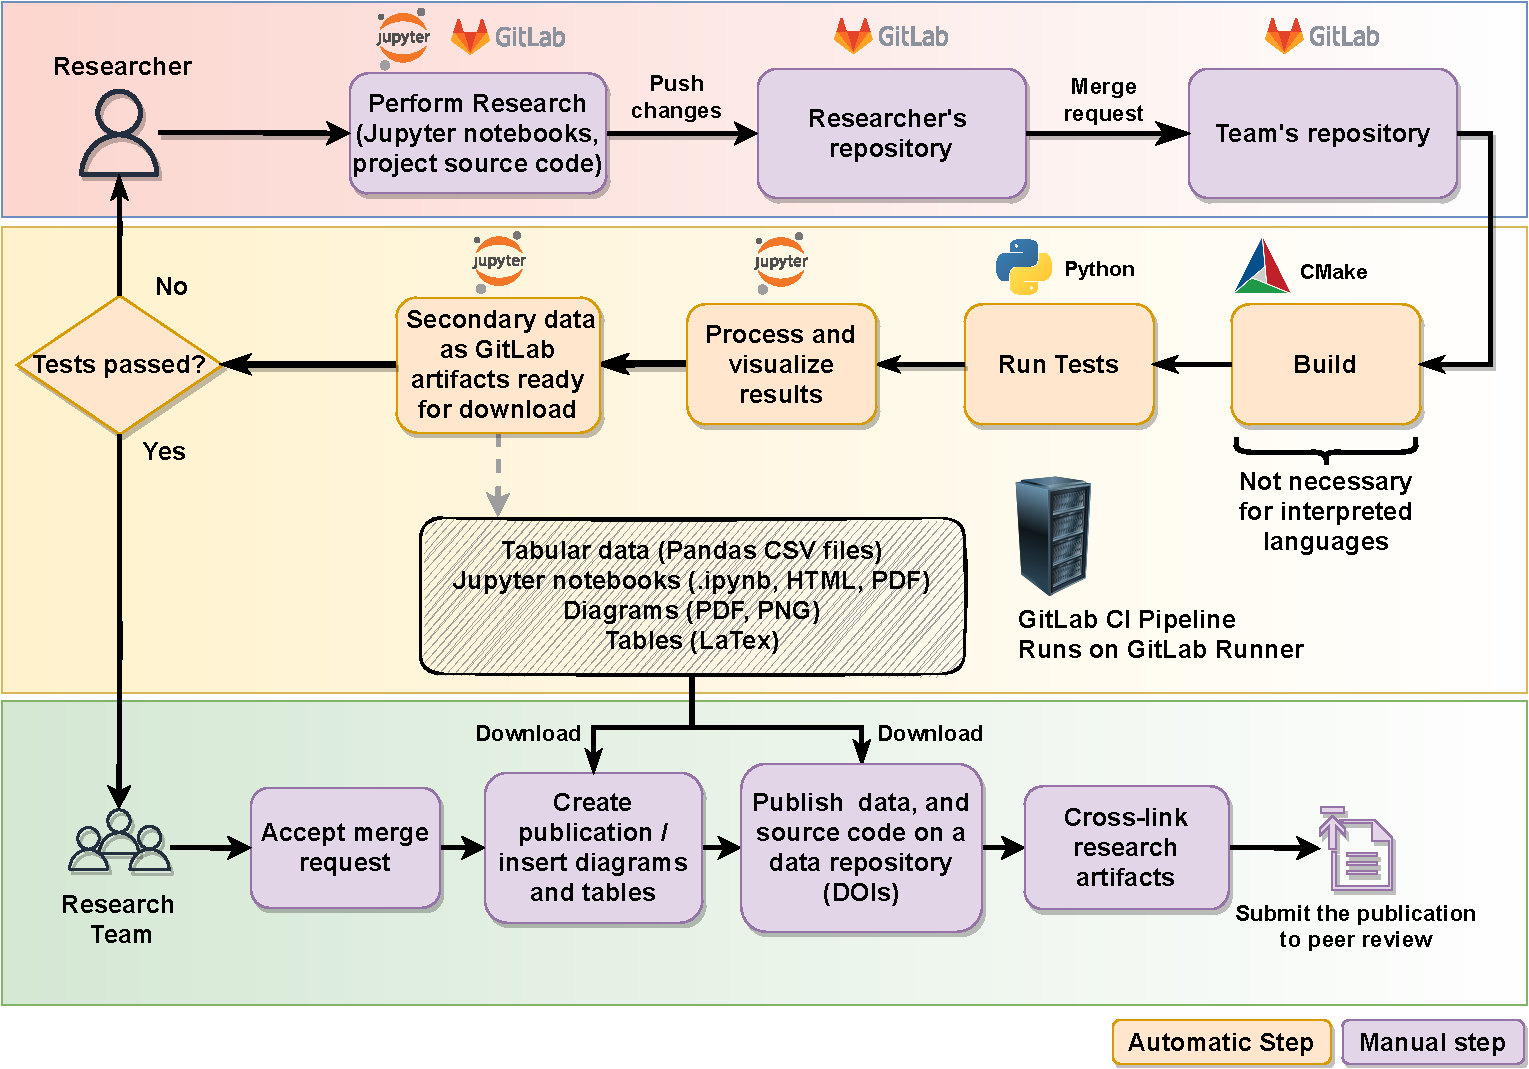
\includegraphics[width=0.8\textwidth]{figures/ZINF-CI-diagram.pdf}

\end{frame}

\begin{frame}{(Continuous Integration with result visualization)} 
    \framesubtitle{Processing and visualizing results}

    \vfill

    \texttt{jupyter nbconvert notebook.ipynb --execute --to FORMAT}

    \medskip

    \begin{itemize}
        \item Execute each jupyter notebook in the repository.
        \item Notebooks agglomerate secondary data into \texttt{pandas.MultiIndex} CSV files. 
        \item Export secondary data and notebooks in different formats as artifacts.
        \item \textbf{Visualization} 
            \begin{itemize}
                \item Download the artifact and open the notebook \faGraduationCap.
                \item \textbf{Alternative:} publish the notebook as a blog post in a GitLab Static Page project. 
                \item Notebooks contain information on failing tests. 
                \item Mapping "caseXYZ" $\to$ "parameter vector" is crucial for re-starting failed parameter variations! 
            \end{itemize}
    \end{itemize}

\end{frame}


\begin{frame}{(Continuous Integration with result visualization)} 
    \framesubtitle{Test evaluation}

    \vfill

    Very straightforward 
    \begin{itemize}
        \item Python scripts test secondary data agglomerated by notebooks from simulation results.
        \item \textbf{Examples:} 
            \begin{itemize}
                \item Is the order of convergence of an error norm $\ge 2.0$?
                \item Is is the difference between simulation and experiment data $\le 4\%$? 
            \end{itemize}
    \end{itemize}

\end{frame}

\begin{frame}{(Continuous Integration with result visualization)} 
    \framesubtitle{Example}

    \vfill
    \begin{center}
        \href{https://gitlab.com/tmaric/fvc-reconstruct/-/pipelines/279564790}{Example OpenFOAM CI project} 
    \end{center}

\end{frame}
